% Options for packages loaded elsewhere
\PassOptionsToPackage{unicode}{hyperref}
\PassOptionsToPackage{hyphens}{url}
%
\documentclass[
]{article}
\usepackage{lmodern}
\usepackage{amssymb,amsmath}
\usepackage{ifxetex,ifluatex}
\ifnum 0\ifxetex 1\fi\ifluatex 1\fi=0 % if pdftex
  \usepackage[T1]{fontenc}
  \usepackage[utf8]{inputenc}
  \usepackage{textcomp} % provide euro and other symbols
\else % if luatex or xetex
  \usepackage{unicode-math}
  \defaultfontfeatures{Scale=MatchLowercase}
  \defaultfontfeatures[\rmfamily]{Ligatures=TeX,Scale=1}
\fi
% Use upquote if available, for straight quotes in verbatim environments
\IfFileExists{upquote.sty}{\usepackage{upquote}}{}
\IfFileExists{microtype.sty}{% use microtype if available
  \usepackage[]{microtype}
  \UseMicrotypeSet[protrusion]{basicmath} % disable protrusion for tt fonts
}{}
\makeatletter
\@ifundefined{KOMAClassName}{% if non-KOMA class
  \IfFileExists{parskip.sty}{%
    \usepackage{parskip}
  }{% else
    \setlength{\parindent}{0pt}
    \setlength{\parskip}{6pt plus 2pt minus 1pt}}
}{% if KOMA class
  \KOMAoptions{parskip=half}}
\makeatother
\usepackage{xcolor}
\IfFileExists{xurl.sty}{\usepackage{xurl}}{} % add URL line breaks if available
\IfFileExists{bookmark.sty}{\usepackage{bookmark}}{\usepackage{hyperref}}
\hypersetup{
  pdftitle={Small Area Estimation for Crime Analysis},
  hidelinks,
  pdfcreator={LaTeX via pandoc}}
\urlstyle{same} % disable monospaced font for URLs
\usepackage[margin=1in]{geometry}
\usepackage{color}
\usepackage{fancyvrb}
\newcommand{\VerbBar}{|}
\newcommand{\VERB}{\Verb[commandchars=\\\{\}]}
\DefineVerbatimEnvironment{Highlighting}{Verbatim}{commandchars=\\\{\}}
% Add ',fontsize=\small' for more characters per line
\usepackage{framed}
\definecolor{shadecolor}{RGB}{248,248,248}
\newenvironment{Shaded}{\begin{snugshade}}{\end{snugshade}}
\newcommand{\AlertTok}[1]{\textcolor[rgb]{0.94,0.16,0.16}{#1}}
\newcommand{\AnnotationTok}[1]{\textcolor[rgb]{0.56,0.35,0.01}{\textbf{\textit{#1}}}}
\newcommand{\AttributeTok}[1]{\textcolor[rgb]{0.77,0.63,0.00}{#1}}
\newcommand{\BaseNTok}[1]{\textcolor[rgb]{0.00,0.00,0.81}{#1}}
\newcommand{\BuiltInTok}[1]{#1}
\newcommand{\CharTok}[1]{\textcolor[rgb]{0.31,0.60,0.02}{#1}}
\newcommand{\CommentTok}[1]{\textcolor[rgb]{0.56,0.35,0.01}{\textit{#1}}}
\newcommand{\CommentVarTok}[1]{\textcolor[rgb]{0.56,0.35,0.01}{\textbf{\textit{#1}}}}
\newcommand{\ConstantTok}[1]{\textcolor[rgb]{0.00,0.00,0.00}{#1}}
\newcommand{\ControlFlowTok}[1]{\textcolor[rgb]{0.13,0.29,0.53}{\textbf{#1}}}
\newcommand{\DataTypeTok}[1]{\textcolor[rgb]{0.13,0.29,0.53}{#1}}
\newcommand{\DecValTok}[1]{\textcolor[rgb]{0.00,0.00,0.81}{#1}}
\newcommand{\DocumentationTok}[1]{\textcolor[rgb]{0.56,0.35,0.01}{\textbf{\textit{#1}}}}
\newcommand{\ErrorTok}[1]{\textcolor[rgb]{0.64,0.00,0.00}{\textbf{#1}}}
\newcommand{\ExtensionTok}[1]{#1}
\newcommand{\FloatTok}[1]{\textcolor[rgb]{0.00,0.00,0.81}{#1}}
\newcommand{\FunctionTok}[1]{\textcolor[rgb]{0.00,0.00,0.00}{#1}}
\newcommand{\ImportTok}[1]{#1}
\newcommand{\InformationTok}[1]{\textcolor[rgb]{0.56,0.35,0.01}{\textbf{\textit{#1}}}}
\newcommand{\KeywordTok}[1]{\textcolor[rgb]{0.13,0.29,0.53}{\textbf{#1}}}
\newcommand{\NormalTok}[1]{#1}
\newcommand{\OperatorTok}[1]{\textcolor[rgb]{0.81,0.36,0.00}{\textbf{#1}}}
\newcommand{\OtherTok}[1]{\textcolor[rgb]{0.56,0.35,0.01}{#1}}
\newcommand{\PreprocessorTok}[1]{\textcolor[rgb]{0.56,0.35,0.01}{\textit{#1}}}
\newcommand{\RegionMarkerTok}[1]{#1}
\newcommand{\SpecialCharTok}[1]{\textcolor[rgb]{0.00,0.00,0.00}{#1}}
\newcommand{\SpecialStringTok}[1]{\textcolor[rgb]{0.31,0.60,0.02}{#1}}
\newcommand{\StringTok}[1]{\textcolor[rgb]{0.31,0.60,0.02}{#1}}
\newcommand{\VariableTok}[1]{\textcolor[rgb]{0.00,0.00,0.00}{#1}}
\newcommand{\VerbatimStringTok}[1]{\textcolor[rgb]{0.31,0.60,0.02}{#1}}
\newcommand{\WarningTok}[1]{\textcolor[rgb]{0.56,0.35,0.01}{\textbf{\textit{#1}}}}
\usepackage{graphicx,grffile}
\makeatletter
\def\maxwidth{\ifdim\Gin@nat@width>\linewidth\linewidth\else\Gin@nat@width\fi}
\def\maxheight{\ifdim\Gin@nat@height>\textheight\textheight\else\Gin@nat@height\fi}
\makeatother
% Scale images if necessary, so that they will not overflow the page
% margins by default, and it is still possible to overwrite the defaults
% using explicit options in \includegraphics[width, height, ...]{}
\setkeys{Gin}{width=\maxwidth,height=\maxheight,keepaspectratio}
% Set default figure placement to htbp
\makeatletter
\def\fps@figure{htbp}
\makeatother
\setlength{\emergencystretch}{3em} % prevent overfull lines
\providecommand{\tightlist}{%
  \setlength{\itemsep}{0pt}\setlength{\parskip}{0pt}}
\setcounter{secnumdepth}{-\maxdimen} % remove section numbering

\title{Small Area Estimation for Crime Analysis}
\author{David Buil-Gil\\
Department of Criminology, University of Manchester, UK}
\date{19/05/2020}

\begin{document}
\maketitle
\begin{abstract}
Victimization surveys provide essential information to study crime and
emotions about crime, but their sampling designs only allow analyzing
criminological variables at large spatial scales. Crime surveys are
designed to allow producing precise direct estimates (i.e., weighted
means and totals) for very large areas, but the size of samples in small
areas is generally small and direct estimates produced for small
geographies will generally be imprecise. Refined model-based small area
estimation techniques may be used to increase the reliability of small
area estimates produced from victimization surveys. Small area
estimation is the term used to describe those methods designed to
produce reliable estimates of parameters of interest (and associated
measures of reliability) for areas for which only small or zero sample
sizes are available. In 2008, the US Panel to Review the Programs of the
Bureau of Justice Statistics recommended the use of small area
estimation to produce subnational estimates of crime. Since then, small
area estimation has been applied to study many variables of interest in
criminology. This chapter introduces theory and a step-by-step exemplar
study in \texttt{R} to show the utility of small area estimation to
analyze crime and place. Model-based regional estimates of confidence in
policing are produced from European Social Survey data.

\par

\textbf{Keywords:} Confidence in policing, European Social Survey, crime
mapping, open data, GIS
\end{abstract}

\textbf{Full reference:} Buil-Gil, D. (2020). Small area estimation for
crime analysis. In E. Groff \& C. Haberman (Eds.), \emph{The study of
crime and place: A methods handbook}. Temple University Press.

\textbf{Contact details:} David Buil-Gil. G18 Humanities Bridgeford
Street Building, Cathie Marsh Institute for Social Research, University
of Manchester. E-mail address:
\emph{\href{mailto:david.builgil@manchester.ac.uk}{\nolinkurl{david.builgil@manchester.ac.uk}}}

\textbf{ORCID ID:} David Buil-Gil: 0000-0002-7549-6317.

\hypertarget{introduction}{%
\section{Introduction}\label{introduction}}

\hypertarget{foundations-of-small-area-estimation}{%
\section{Foundations of small area
estimation}\label{foundations-of-small-area-estimation}}

\hypertarget{small-area-estimation-applications-for-crime-analysis}{%
\section{Small area estimation applications for crime
analysis}\label{small-area-estimation-applications-for-crime-analysis}}

\hypertarget{producing-small-area-estimates-of-confidence-in-the-police-step-by-step-example-in-r}{%
\section{\texorpdfstring{Producing small area estimates of confidence in
the police: Step-by-step example in
\texttt{R}}{Producing small area estimates of confidence in the police: Step-by-step example in R}}\label{producing-small-area-estimates-of-confidence-in-the-police-step-by-step-example-in-r}}

\hypertarget{european-social-survey}{%
\subsection{European Social Survey}\label{european-social-survey}}

The European Social Survey is a biannual cross-national survey designed
to measure social attitudes, beliefs and behaviors. It has been
conducted since 2001 in more than 35 European countries, and allows for
cross-national and cross-sectional comparisons of crime-related issues
such as the confidence in police services, worry about crime and crime
victimization experience in the last 5 years. The ESS sample is designed
to be representative of all individual residents aged 15 or older who
live in private households in each participant country, regardless of
their nationality, citizenship or language.

Although participant countries are responsible for producing their own
national sampling designs, all counties must collow common sampling
principles. Namely, respondents must be selected following strict random
probability techniques at every stage, sampling frames can be
individuals, households or addresses, quota sampling is not allowed, and
non-responding units cannot be replaced. Moreover, every country must
select at least 1,500 effective respondents (or at least 800 in
participant countries with less than 2 million citizens). As a
consequence, countries with very different number of residents may
select similar sample sizes, and all geographical levels below countries
(e.g., regions, counties, cities) are not planned by the original
sampling design and record small sample sizes.

\hypertarget{download-european-social-survey-data}{%
\subsubsection{Download European Social Survey
data}\label{download-european-social-survey-data}}

ESS data can be downloaded from their website. But we can also download
ESS data direcly into our \texttt{R} system using the \texttt{essurvey}
package developed by Cimentada (2019). This package is designed to
facilitate loading ESS survey data into \texttt{R}. It allows users to
select the countries and years they are interested to analyze and
loading them directly in \texttt{R} If this is the first time we are
using this package, we need to install it by using the
\texttt{install.packages()} function.

\begin{Shaded}
\begin{Highlighting}[]
\KeywordTok{install.packages}\NormalTok{(}\StringTok{"essurvey"}\NormalTok{) }
\end{Highlighting}
\end{Shaded}

Once it is installed, we can load the package into our \texttt{R}
environment using the \texttt{library()} function.

\begin{Shaded}
\begin{Highlighting}[]
\KeywordTok{library}\NormalTok{(essurvey)}
\end{Highlighting}
\end{Shaded}

In order to access ESS data in \texttt{R}, first we need to create our
own personal account in the ESS online portal. ESS users only need to
registed once, and then they can have open access to ESS data as many
times as they wish. We need to access the ESS website and create a new
account with our personal details:
\url{https://www.europeansocialsurvey.org/user/new}. Filling the online
registration form takes less than one minute, and once it is completed
we will receive an email to confirm our registration process.

Once we are registered in the ESS platform, we can direcly import all
ESS data into \texttt{R}. In this exercise we will download and analyze
data from the 8th edition of ESS, which was published in 2016. We use
the function \texttt{set\_email()} from \texttt{essurvey} to save our
email (the email account registered in the ESS platform) as a new
environment variable, and then run the \texttt{import\_rounds()}
function to load ESS data from all participant countries. This may take
a few seconds.

\begin{Shaded}
\begin{Highlighting}[]
\KeywordTok{set_email}\NormalTok{(}\StringTok{"your_email@domain.com"}\NormalTok{) }\CommentTok{# change by your email}

\NormalTok{ess <-}\StringTok{ }\KeywordTok{import_rounds}\NormalTok{(}\DataTypeTok{rounds =} \DecValTok{8}\NormalTok{, }\DataTypeTok{ess_email =} \OtherTok{NULL}\NormalTok{, }\DataTypeTok{format =} \OtherTok{NULL}\NormalTok{)}
\end{Highlighting}
\end{Shaded}

Now we have loaded the ESS data and we can begin exploring and analyzing
it. If we want to see the data, we can use the \texttt{View()} function.

\hypertarget{descriptive-analyses}{%
\subsection{Descriptive analyses}\label{descriptive-analyses}}

The ESS includes various questions that may be of interest for
criminologists and crime analysts. For examples, some questions that we
may be interested to analyze are:

\textbf{1.-} \emph{``Have you or a member of your household been the
victim of a burglary or assault in the last 5 years?''} \textbf{2.-}
\emph{``How safe do you -- or would you -- feel walking alone in this
area after dark?''} \textbf{3.-} \emph{``Using this card, please tell me
on a score of 0-10 how much you personally trust each of the
institutions I read out {[}\ldots{]}''; ``{[}\ldots{]} the legal
system'' and ``{[}\ldots{]} the police''.}

These measures have previously been used to study victimization,
perceived safety, trust in the police, and trust in the legal system
(e.g., REFS), but there are many other questions that may also be of
interest for criminologists (e.g., racism, discrimination against
immigrants, homophobia). We can read the whole ESS questionnaire here:
\url{https://www.europeansocialsurvey.org/docs/round8/fieldwork/source/ESS8_source_questionnaires.pdf}.

In this exemplar study we will analyze ESS data about trust in police
services, following previous research conducted by REFS. The variable
name is \texttt{trstplc}, and it a Likert scale variable from 0 to 10,
where 0 indicates the lowest level of trust, and 10 is the maximum
value. We can begin by checking how this measure of trust in the police
looks like. We will use the \texttt{summary()} function to obtain the
summary statistics of this variable.

\begin{Shaded}
\begin{Highlighting}[]
\KeywordTok{summary}\NormalTok{(ess}\OperatorTok{$}\NormalTok{trstplc)}
\end{Highlighting}
\end{Shaded}

\begin{verbatim}
##    Min. 1st Qu.  Median    Mean 3rd Qu.    Max.    NA's 
##   0.000   5.000   7.000   6.399   8.000  10.000     320
\end{verbatim}

We see that the average score of trust in police in Europe is 6.4, and
the median value is 7. We can use the same \texttt{summary()} function
to compare the values of trust in police services with the citizens'
trust in other social institutions, such as the legal system (variable
\texttt{trstlgl}), politicians (\texttt{trtplt}), political parties
(\texttt{trtprt}), the country's parliament (\texttt{trstprl}) or the
United Nations (\texttt{trstun}). On average, we measures of trust in
the police appear to be higher than the Europeans' trust in other key
political and legal institutions.

Moreover, we can obtain some more detailed information about the
citizens' trust in police services by counting the frequency of
respondents that chose each score and creating a bar plot to visualize
their distribution. We will use functions from the the packages
\texttt{dplyr} (Wickham, François, et al., 2020) and \texttt{ggplot2}
(Wickham, Chang, et al., 2020) for this. More specifically, we use the
\texttt{group\_by()} function from \texttt{dplyr} to create groups of
respondents based on their score of trust in police, and the functions
\texttt{summarize()} and \texttt{mutate()} from the same package to save
the results in two columns showing the number and proportion of
respondents in each category. We save this new table in a new dataset
called \texttt{trust\_poli}.

\begin{Shaded}
\begin{Highlighting}[]
\NormalTok{trust_poli <-}\StringTok{ }\NormalTok{ess }\OperatorTok
\StringTok{  }\KeywordTok{group_by}\NormalTok{(trstplc) }\OperatorTok\StringTok{     }\CommentTok{# categories based on level of trust}
\StringTok{  }\KeywordTok{summarize}\NormalTok{(}\DataTypeTok{n =} \KeywordTok{n}\NormalTok{()) }\OperatorTok\StringTok{    }\CommentTok{# number of respondents per group}
\StringTok{  }\KeywordTok{mutate}\NormalTok{(}\DataTypeTok{prop =}\NormalTok{ n }\OperatorTok{/}\StringTok{ }\KeywordTok{sum}\NormalTok{(n)) }\CommentTok{# proportion respondents per group}
\end{Highlighting}
\end{Shaded}

Then, we use the \texttt{ggplot()} and \texttt{geom\_bar()} functions
from \texttt{ggplot2} to create a bar graph of the number of responses
per category. Before plotting this visualization, however, we will run
the function \texttt{theme\_set(theme\_minimal())} to set a basic, neat
theme for all our plots.

\begin{Shaded}
\begin{Highlighting}[]
\KeywordTok{theme_set}\NormalTok{(}\KeywordTok{theme_minimal}\NormalTok{()) }\CommentTok{# set white theme for plots}

\KeywordTok{ggplot}\NormalTok{(}\DataTypeTok{data =}\NormalTok{ trust_poli, }\KeywordTok{aes}\NormalTok{(}\DataTypeTok{x =}\NormalTok{ trstplc, }\DataTypeTok{y =}\NormalTok{ prop)) }\OperatorTok{+}\StringTok{ }\CommentTok{# set variables of interest}
\StringTok{  }\KeywordTok{geom_bar}\NormalTok{(}\DataTypeTok{stat=}\StringTok{"identity"}\NormalTok{) }\OperatorTok{+}\StringTok{                           }\CommentTok{# plot bar graph}
\StringTok{  }\KeywordTok{ggtitle}\NormalTok{(}\StringTok{"Trust in police across European countries"}\NormalTok{)  }\CommentTok{# change title}
\end{Highlighting}
\end{Shaded}

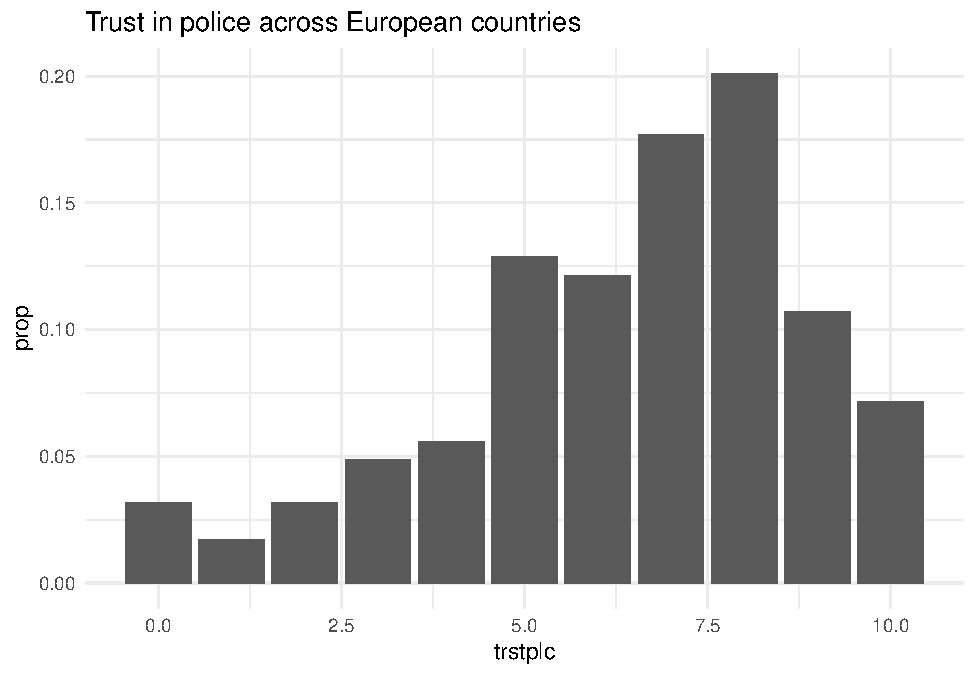
\includegraphics{chapter_files/figure-latex/plot trust police-1.pdf}

We see that few respondents have a low trust in the police, whereas most
European citizens seem to trust their police forces quite a lot. This
plot, nevertheless, may hide internal heterogeneity between European
regions and countries. Based on this bar graph alone, we do not have
enough information to be able to know if residents in all participant
countries have the similar levels of trust in the police, or whether
those respondents with very low or very high confidence in the police
concentrate in some countries but not others. We will use small area
estimation to produce estimates of trust in the police across European
regions.

Since we are particularly interested in analyzing which regions in
Europe have more and less trust in police services, and not only what is
the level of trust in each area, we will produce regional estimates of
the proportion of citizens who have a level of trust above the average
in Europe. In other words, our estimates will show a value between 0 and
1 representing which proportion of residents have more trust in the
police than the average of European citizens. For instance, a value of
0.6 in a given region would indicate that 60 percent of its residents
have more trust in the police than the European average. Thus, we need
to recode our variable of interest, and we will use the
\texttt{mutate()} and \texttt{ifelse()} functions from \texttt{dplyr} to
do so. Those respondents with a score above or equal to the mean will be
given a value 1, whereas others will be assigned a value of 0. This will
facilitate the interpretation of our results, but future research can
explore producing estimates from the original 0-to-10 Likert scale. We
will also delete all those respondents who did not answer this question
(i.e., \emph{NA}s).

\begin{Shaded}
\begin{Highlighting}[]
\NormalTok{ess <-}\StringTok{ }\NormalTok{ess }\OperatorTok
\StringTok{  }\CommentTok{# if trust is above or equal to mean, 1, 0}
\StringTok{  }\KeywordTok{mutate}\NormalTok{(}\DataTypeTok{trstplc =} \KeywordTok{ifelse}\NormalTok{(trstplc }\OperatorTok{>=}\StringTok{ }\KeywordTok{mean}\NormalTok{(trstplc, }\DataTypeTok{na.rm =}\NormalTok{ T), }\DecValTok{1}\NormalTok{, }\DecValTok{0}\NormalTok{)) }\OperatorTok
\StringTok{  }\KeywordTok{filter}\NormalTok{(}\OperatorTok{!}\KeywordTok{is.na}\NormalTok{(trstplc)) }\CommentTok{# delete NAs}
\end{Highlighting}
\end{Shaded}

We can use the \texttt{group\_by()} and \texttt{summarize()} functions
seen above to explore how our recoded variable looks like. We can see,
for example, that 24721 out of 44067 (i,e., 56.1\% of participants) have
more trust in the police than the average in Europe.

\hypertarget{exploring-spatial-data-coverage-and-sample-sizes}{%
\subsection{Exploring spatial data: Coverage and sample
sizes}\label{exploring-spatial-data-coverage-and-sample-sizes}}

As mentioned above, the ESS sampling design is planned to allow
producing reliable direct estimates at the level participant countries,
but samples recorded at smaller scales (e.g., regions, cities) may be
too small in some areas to allow producing direct estimates of adequate
precision. We can check how big ESS sample sizes are in each region
(variable \texttt{region}) using the functions \texttt{filter()},
\texttt{group\_by()} and \texttt{summarize()} from \texttt{dplyr} to
create a summary table in a new dataframe that we will call
\texttt{sample\_region}. Then, we can use the \texttt{summary()}
function to print the summary statistics of area sample sizes.

\begin{Shaded}
\begin{Highlighting}[]
\NormalTok{sample_region <-}\StringTok{ }\NormalTok{ess }\OperatorTok
\StringTok{  }\KeywordTok{filter}\NormalTok{(region }\OperatorTok{!=}\StringTok{ }\DecValTok{99999}\NormalTok{) }\OperatorTok\StringTok{ }\CommentTok{# filter out NAs}
\StringTok{  }\KeywordTok{group_by}\NormalTok{(region) }\OperatorTok\StringTok{        }\CommentTok{# categories based on regions}
\StringTok{  }\KeywordTok{summarize}\NormalTok{(}\DataTypeTok{n =} \KeywordTok{n}\NormalTok{())          }\CommentTok{# calculate sample size}

\KeywordTok{summary}\NormalTok{(sample_region}\OperatorTok{$}\NormalTok{n)}
\end{Highlighting}
\end{Shaded}

\begin{verbatim}
##    Min. 1st Qu.  Median    Mean 3rd Qu.    Max. 
##     7.0    60.0   115.0   160.8   209.8  2524.0
\end{verbatim}

The average sample size per region is 160.8, which is quite large but
may be insufficient to produce reliable direct estimates. Moreover,
there are areas with very small sample sizes (the minimum area sample
size is 7), where we cannot simply rely of direct estimation techiques
to generate estimates of adequate precision.

Moreover, we also need to consider that participant countries can decide
whether they want to publish recorded data at the level of NUTS-1,
NUTS-2, NUTS-3 or smaller scales. NUTS is the acronym of
\emph{Nomenclature of Territorial Units for Statistics}, and it refers
to the spatial scales used by the European Union and Eurostat (the
statistical office of the European Union) for policy making and
statistical reporing purposes. NUTS are basically a way to organize
European countries in regions and subregions. In England, for instance
NUTS-1 are statistical regions, NUTS-2 are counties (and groups of
districts in London), and NUTS-3 are generally unitary authorities (some
grouped). Whereas some participant countries publish their data at the
level of NUTS-2, others decide to report information for NUTS-1 or
NUTS-3 areas. We can check which level of aggregation is published by
each participant country in the ESS website:
\url{https://www.europeansocialsurvey.org/data/multilevel/guide/essreg.html}.
We can also run the following lines of code and print this information
directly in \texttt{R}.

\begin{Shaded}
\begin{Highlighting}[]
\NormalTok{ess }\OperatorTok
\StringTok{  }\KeywordTok{group_by}\NormalTok{(regunit, cntry) }\OperatorTok\StringTok{ }\CommentTok{# group by spatial scale and country}
\StringTok{  }\KeywordTok{summarize}\NormalTok{(}\DataTypeTok{n =} \KeywordTok{n}\NormalTok{())           }\CommentTok{# print sample size per country}
\end{Highlighting}
\end{Shaded}

We see that many counties publish data at the NUTS-2 level, but others
participant countries publish their micro-data for NUTS-1 and NUTS-3
areas. We will aggregate data at the NUTS-2 level and produce estimates
of confidence in the police at this scale (with the exception of Germany
and the UK, who only publish data for NUTS-1).

\hypertarget{converting-spatial-data-into-nuts-2}{%
\subsubsection{Converting spatial data into
NUTS-2}\label{converting-spatial-data-into-nuts-2}}

In order to convert the spatial information provided by all countries
into NUTS-2 geographies, we first need to load a lookup table that
details which NUTS-3 areas are part of which NUTS-2. I have previously
created and saved a lookup table in csv format in an open access Github
repository, but similar tables are also available in other formats from
the ESS platform:
\url{https://www.europeansocialsurvey.org/data/multilevel/guide/bulk.html}.
In order to load the lookup table in \texttt{R}, we can use the
\texttt{getURL()} functions from \texttt{RCurl} {[}ADD REF{]} and
\texttt{read.csv()}.

\begin{Shaded}
\begin{Highlighting}[]
\KeywordTok{library}\NormalTok{(RCurl)}

\NormalTok{url_lookup <-}\StringTok{ }\KeywordTok{getURL}\NormalTok{(}\StringTok{"https://raw.githubusercontent.com/davidbuilgil/SAE_chapter/master/data/NUTS_lookup.csv"}\NormalTok{)}

\NormalTok{lookup <-}\StringTok{ }\KeywordTok{read.csv}\NormalTok{(}\DataTypeTok{text =}\NormalTok{ url_lookup)}
\end{Highlighting}
\end{Shaded}

Now, we can create a new column in the original ESS data that specifies
the regions for which we aim to produce small area estimates of trust in
the police. We will merge the lookup table with the original ESS data
using a \texttt{left\_join()} function and create a new column called
\texttt{domain} which shows the NUTS-2 areas (or NUTS-1 in Germany and
UK) for which we will produce estimates.

\begin{Shaded}
\begin{Highlighting}[]
\NormalTok{ess <-}\StringTok{ }\NormalTok{ess}\OperatorTok
\StringTok{  }\KeywordTok{left_join}\NormalTok{(lookup, }\DataTypeTok{by =} \KeywordTok{c}\NormalTok{(}\StringTok{"region"}\NormalTok{ =}\StringTok{ "nuts3"}\NormalTok{)) }\OperatorTok\StringTok{          }\CommentTok{# merge lookup into ESS dataset}
\StringTok{  }\KeywordTok{rename}\NormalTok{(}\DataTypeTok{domain =}\NormalTok{ nuts2) }\OperatorTok\StringTok{                                 }\CommentTok{# rename NUTS2 variable}
\StringTok{  }\KeywordTok{mutate}\NormalTok{(}\DataTypeTok{domain =} \KeywordTok{as.character}\NormalTok{(domain),                      }\CommentTok{# convert NUTS2 into character}
         \DataTypeTok{domain =} \KeywordTok{ifelse}\NormalTok{(}\KeywordTok{is.na}\NormalTok{(domain), region, domain)) }\OperatorTok\StringTok{ }\CommentTok{# copy NUTS1 data if no NUTS2 information}
\StringTok{  }\KeywordTok{filter}\NormalTok{(}\OperatorTok{!}\NormalTok{(domain }\OperatorTok{==}\StringTok{ }\DecValTok{99999}\NormalTok{))                                 }\CommentTok{# delete NAs}
\end{Highlighting}
\end{Shaded}

Now our data is clean and ready to be used to produce estimates of trust
in the police at a regional level.

\hypertarget{producing-direct-estimates}{%
\subsection{Producing direct
estimates}\label{producing-direct-estimates}}

We will produce direct estimates based on the Horvitz-Thompson estimator
(Horvitz \& Thompson, 1952), which is one of the most common approaches
to produce direct estimates. It makes use of original survey data and
survey weights to obtain design-unbiased estimates in each small area,
but direct estimates may suffer from high variance and unreliability in
those areas with small sample sizes. Moreover, estimates cannot be
produced in areas with zero samples. We will produce Horvitz-Thompson
estimates of the trust in police for European regions, but it is very
likely than many estimators will not show adequate levels of precision.
Model-based SAE approaches are needed when direct estimates are not
precise enough.

In order to produce small area estimates, we will use the \texttt{sae}
package {[}REFS{]}. We need to install it and load it into your
\texttt{R} system.

\begin{Shaded}
\begin{Highlighting}[]
\KeywordTok{library}\NormalTok{(sae)}
\end{Highlighting}
\end{Shaded}

The Horvitz-Thompson estimator takes into account the population size in
each area, and assumes that survey weights adjust our sample to the
total population. Thus, we need to know how many people live in each
region, and ensure that our weights adjust the sample to the population
size. I have previously downloaded the population sizes from Eurostat
and uploaded a clean dataset onto Github. Downloading data from sources
of official statistics, such as Eurostat, usually mean having to spend
some time cleaning the data and selecting those variables that adjust to
our research needs. For the purpose of this exercise, I have cleaned the
data and uploaded onto an online repository, but later we will also see
how to load Eurostat data into our \texttt{R} environments.

\begin{Shaded}
\begin{Highlighting}[]
\NormalTok{url_pop <-}\StringTok{ }\KeywordTok{getURL}\NormalTok{(}\StringTok{"https://raw.githubusercontent.com/davidbuilgil/SAE_chapter/master/data/population.csv"}\NormalTok{)}

\NormalTok{pop <-}\StringTok{ }\KeywordTok{read.csv}\NormalTok{(}\DataTypeTok{text =}\NormalTok{ url_pop)}
\end{Highlighting}
\end{Shaded}

\begin{Shaded}
\begin{Highlighting}[]
\NormalTok{pop <-}\StringTok{ }\NormalTok{pop }\OperatorTok
\StringTok{  }\KeywordTok{mutate}\NormalTok{(}\DataTypeTok{area =} \DecValTok{1}\OperatorTok{:}\KeywordTok{n}\NormalTok{()) }\OperatorTok\StringTok{                 }\CommentTok{# create numeric id value}
\StringTok{  }\KeywordTok{rename}\NormalTok{(}\StringTok{"domain"}\NormalTok{ =}\StringTok{ "X.U.FEFF.domain"}\NormalTok{) }\OperatorTok\StringTok{ }\CommentTok{# rename region column name}
\StringTok{  }\KeywordTok{subset}\NormalTok{(}\DataTypeTok{select =} \KeywordTok{c}\NormalTok{(}\DecValTok{1}\NormalTok{, }\DecValTok{3}\NormalTok{, }\DecValTok{2}\NormalTok{)) }\OperatorTok\StringTok{          }\CommentTok{# reorder columns}
\StringTok{  }\KeywordTok{filter}\NormalTok{(domain }\OperatorTok\StringTok{ }\NormalTok{ess}\OperatorTok{$}\NormalTok{domain)           }\CommentTok{# filter out areas not present in ESS}
\end{Highlighting}
\end{Shaded}

Now we have almost all information necessary to produce our direct
estimates: the variable of interest (variable \texttt{trstplc} in the
\texttt{ess} dataset), the area population size (\texttt{pop2014} in
\texttt{pop} dataset), and spatial information that matches in both
datasets. Nevertheless, as introduced above, the Horvitz-Thompson
estimator also requires the use of survey weights that adjust our sample
to the population size. Given that the weights published by ESS are not
designed to let respondents represent a specific number of citizens, but
instead they were computed to adjust the sample to the population
characteristics, we will need to recalibrate the ESS weights to the
population sizes per region. We can do this by running the following
lines of code:

\begin{Shaded}
\begin{Highlighting}[]
\NormalTok{ess_w_area <-}\StringTok{ }\NormalTok{ess }\OperatorTok
\StringTok{  }\KeywordTok{filter}\NormalTok{(domain }\OperatorTok\StringTok{ }\NormalTok{pop}\OperatorTok{$}\NormalTok{domain) }\OperatorTok\StringTok{        }\CommentTok{# filter out areas not present in population dataset}
\StringTok{  }\KeywordTok{group_by}\NormalTok{(domain) }\OperatorTok\StringTok{                      }\CommentTok{# create groups by region}
\StringTok{  }\KeywordTok{summarise}\NormalTok{(}\DataTypeTok{w_sum =} \KeywordTok{sum}\NormalTok{(pspwght }\OperatorTok{*}\StringTok{ }\NormalTok{pweight)) }\CommentTok{# sum weights per region}

\NormalTok{ess <-}\StringTok{ }\NormalTok{ess }\OperatorTok
\StringTok{  }\KeywordTok{filter}\NormalTok{(domain }\OperatorTok\StringTok{ }\NormalTok{pop}\OperatorTok{$}\NormalTok{domain) }\OperatorTok\StringTok{          }\CommentTok{# filter out areas not present in population dataset}
\StringTok{  }\KeywordTok{left_join}\NormalTok{(ess_w_area, }\DataTypeTok{by =} \StringTok{"domain"}\NormalTok{) }\OperatorTok\StringTok{    }\CommentTok{# merge sum of weights with ESS units }
\StringTok{  }\KeywordTok{left_join}\NormalTok{(pop, }\DataTypeTok{by =} \StringTok{"domain"}\NormalTok{) }\OperatorTok\StringTok{           }\CommentTok{# merge region population sizes}
\StringTok{  }\KeywordTok{mutate}\NormalTok{(}\DataTypeTok{weight =}\NormalTok{ pspwght }\OperatorTok{*}\StringTok{ }\NormalTok{pweight,          }\CommentTok{# compute weights for cross-national analysis}
         \DataTypeTok{weight =}\NormalTok{ (weight }\OperatorTok{*}\StringTok{ }\NormalTok{pop2016) }\OperatorTok{/}\StringTok{ }\NormalTok{w_sum) }\CommentTok{# recalibrate weights to population sample size}
\end{Highlighting}
\end{Shaded}

After a few steps, we now have all necessary information to produce our
direct estimates of confidence in policing. We use the \texttt{direct()}
function from \texttt{sae} to produce Horvitz-Thompson estimates in each
region. It will also produce the Coefficient of Variation of each
estimate, which will be used to assess the reliability of these direct
estimates.

\begin{Shaded}
\begin{Highlighting}[]
\NormalTok{dir <-}\StringTok{ }\KeywordTok{direct}\NormalTok{(}\DataTypeTok{y       =}\NormalTok{ ess}\OperatorTok{$}\NormalTok{trstplc,}
              \DataTypeTok{dom     =}\NormalTok{ ess}\OperatorTok{$}\NormalTok{area,}
              \DataTypeTok{sweight =}\NormalTok{ ess}\OperatorTok{$}\NormalTok{weight,}
              \DataTypeTok{domsize =}\NormalTok{ pop[,}\DecValTok{2}\OperatorTok{:}\DecValTok{3}\NormalTok{],}
              \DataTypeTok{replace =} \OtherTok{FALSE}\NormalTok{)}
\end{Highlighting}
\end{Shaded}

\hypertarget{exploring-direct-estimates}{%
\subsubsection{Exploring direct
estimates}\label{exploring-direct-estimates}}

Once we have produced our direct estimates of trust in the police, we
can see how these look like by using some functions introduced above.

\begin{Shaded}
\begin{Highlighting}[]
\KeywordTok{summary}\NormalTok{(dir}\OperatorTok{$}\NormalTok{Direct) }\CommentTok{# summary statistics of direct estimates}
\end{Highlighting}
\end{Shaded}

\begin{verbatim}
##    Min. 1st Qu.  Median    Mean 3rd Qu.    Max. 
##  0.1783  0.4877  0.5815  0.5838  0.6704  0.9006
\end{verbatim}

\begin{Shaded}
\begin{Highlighting}[]
\CommentTok{# produce boxplot of coefficients of variation}
\KeywordTok{ggplot}\NormalTok{(dir, }\KeywordTok{aes}\NormalTok{(}\DataTypeTok{x=}\NormalTok{Domain, }\DataTypeTok{y=}\NormalTok{CV)) }\OperatorTok{+}\StringTok{ }
\StringTok{  }\KeywordTok{geom_boxplot}\NormalTok{() }\OperatorTok{+}
\StringTok{  }\KeywordTok{ggtitle}\NormalTok{(}\StringTok{"Coefficient of Variation of direct estimates"}\NormalTok{)}
\end{Highlighting}
\end{Shaded}

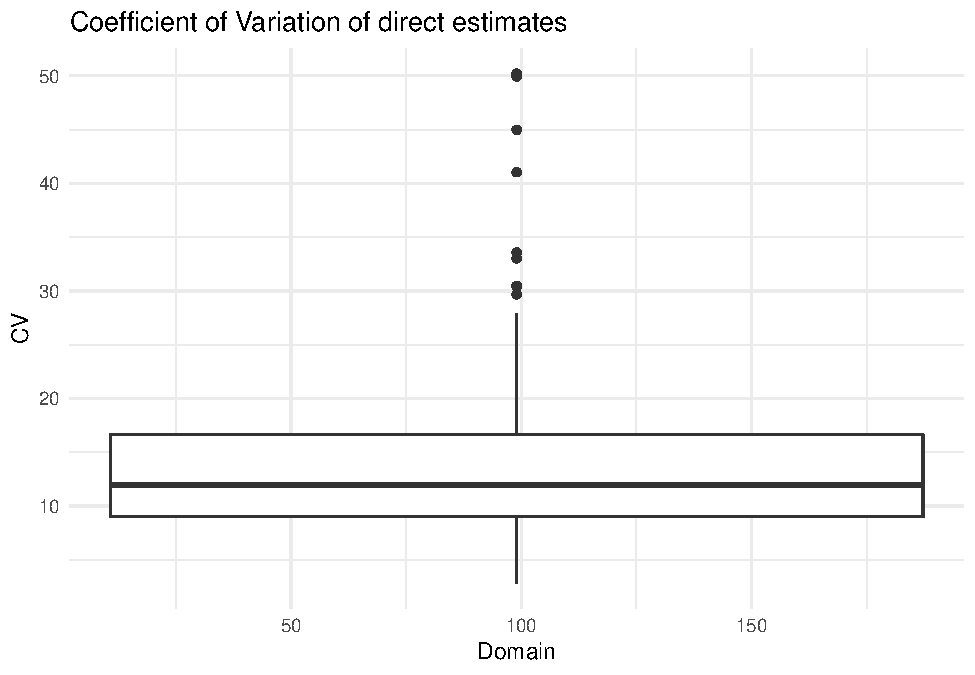
\includegraphics{chapter_files/figure-latex/dir cv boxplot-1.pdf}

As you can see in the boxplot, the estimates of the majority of regions
have a Coefficient of Variation smaller than 20\%, which is a very good
indicator of reliability of these estimates; but we also have a few
regions with Coefficients of Variation larger than 25\%. We can improve
the accuracy of these estimates by using model-based small area
estimation models.

For now, we can merge our direct estimates into the dataset of
area-level information by using the \texttt{left\_join()} function from
`dplyr.

\begin{Shaded}
\begin{Highlighting}[]
\NormalTok{pop <-}\StringTok{ }\NormalTok{pop }\OperatorTok
\StringTok{  }\KeywordTok{left_join}\NormalTok{(dir, }\DataTypeTok{by =} \KeywordTok{c}\NormalTok{(}\StringTok{"area"}\NormalTok{ =}\StringTok{ "Domain"}\NormalTok{))}
\end{Highlighting}
\end{Shaded}

\hypertarget{downloading-area-level-covariates}{%
\subsection{Downloading area-level
covariates}\label{downloading-area-level-covariates}}

In order to fit area-level models of trust in police and produce
area-level estimates, we will need area-level covariates that are
associated with our variable of interest. ADD SOME LITERATURE ON
COVARIATES!!!

We can download various area-level covariates from Eurostat using the
\texttt{eurostat} package (Lahti et al., 2020), which has been created
by facilitate downloading data from Eurostat into \texttt{R}. Eurostat
is a very large data repository that publishes large datasets of social,
econonomic and demographic information for European countries and
regions. We can use the \texttt{search\_eurostat()} function to search
predefined key words associated with variables of interest for our
study. The function will return a list of all datasets including our
keywords, and can then explore which of them are more suitable for our
study. For example, we may want to know if education levels and crime
rates are somehow associated with the regional levels of trust in the
police, and thus we can search Eurostat datasets that include the words
\emph{``education''} and \emph{``offender''}. I have done this search
and found various variables of interest, but you can also try this at
home and probably you will also find variables of interest for our
models.

\begin{Shaded}
\begin{Highlighting}[]
\KeywordTok{library}\NormalTok{(eurostat)}

\NormalTok{eurostat_edu   <-}\StringTok{ }\KeywordTok{search_eurostat}\NormalTok{(}\StringTok{"education"}\NormalTok{) }\CommentTok{# search datasets about education}
\NormalTok{eurostat_crime <-}\StringTok{ }\KeywordTok{search_eurostat}\NormalTok{(}\StringTok{"offender"}\NormalTok{)  }\CommentTok{# search datasets about crime}
\end{Highlighting}
\end{Shaded}

Once we know the codes of the datasets we are interested to do, we can
use the \texttt{get\_eurostat()} function to import these into our
\texttt{R} environment. For example, the dataset
\texttt{edat\_lfs\_9918} includes information about the proportion of
citizens between 15 and 64 in each NUTS-2 that have a higher education
degree. We can download this dataset and see how it looks like:

\begin{Shaded}
\begin{Highlighting}[]
\NormalTok{he <-}\StringTok{ }\KeywordTok{get_eurostat}\NormalTok{(}\DataTypeTok{id =} \StringTok{"edat_lfs_9918"}\NormalTok{)}
\end{Highlighting}
\end{Shaded}

If we open this file (using the \texttt{View()} function), we can see
that it is includes information about many indicators, years, age
groups, spatial scales and divided by sex. All datasets imported from
Eurostat provide information abou many different measures, which means
that we will need to spend some time wrangling and subsetting these data
to make sure we can attach these to our area-level direct estimates to
estimate the area-level models needed to produce model-based estimates.
For the purpose of this exemplar study, I have previously searched for
datasets of interest, downloaded and cleaned their data, and merged all
covariates into a unique dataset. We can load this dataset into
\texttt{R} using the functions provided by \texttt{RCurl} package, but
you can also spend some time trying to find better, more suitable
covariates in the Eurostat website. Moreover, the ESS website also
publishes interesting area-level covariates at the different scales:
\url{https://www.europeansocialsurvey.org/data/multilevel/guide/bulk.html}.

\begin{Shaded}
\begin{Highlighting}[]
\NormalTok{url_covs <-}\StringTok{ }\KeywordTok{getURL}\NormalTok{(}\StringTok{"https://raw.githubusercontent.com/davidbuilgil/SAE_chapter/master/data/covs_short.csv"}\NormalTok{)}

\NormalTok{covs <-}\StringTok{ }\KeywordTok{read.csv}\NormalTok{(}\DataTypeTok{text =}\NormalTok{ url_covs)}

\NormalTok{pop <-}\StringTok{ }\NormalTok{pop }\OperatorTok
\StringTok{  }\KeywordTok{left_join}\NormalTok{(covs, }\DataTypeTok{by =} \StringTok{"domain"}\NormalTok{) }\CommentTok{# merge covariates with direct estimates}
\end{Highlighting}
\end{Shaded}

rate crimes * 10000

Describe variables like this: - \emph{BLA}: bla bla bla

Once all our covariates are clean and ready to use, we can briefly
explore them using the \texttt{dplyr} package. For instance, we may want
to know the number of missing values in each covariate:

\begin{Shaded}
\begin{Highlighting}[]
\NormalTok{pop }\OperatorTok
\StringTok{  }\NormalTok{dplyr}\OperatorTok{::}\KeywordTok{select}\NormalTok{(fem_p_}\DecValTok{16}\NormalTok{, gdp_eurhab_}\DecValTok{16}\NormalTok{, robb_r_}\DecValTok{10}\NormalTok{, burg_r_}\DecValTok{10}\NormalTok{, he_p_}\DecValTok{16}\NormalTok{, medage_}\DecValTok{16}\NormalTok{) }\OperatorTok
\StringTok{  }\KeywordTok{summarise_all}\NormalTok{(}\KeywordTok{funs}\NormalTok{(}\KeywordTok{sum}\NormalTok{(}\KeywordTok{is.na}\NormalTok{(.))))}
\end{Highlighting}
\end{Shaded}

\begin{verbatim}
##   fem_p_16 gdp_eurhab_16 robb_r_10 burg_r_10 he_p_16 medage_16
## 1        0            13        22        22      10        10
\end{verbatim}

\hypertarget{impute-missing-values}{%
\subsubsection{Impute missing values}\label{impute-missing-values}}

Multiple Imputation using Bootstrap and PMM

\begin{Shaded}
\begin{Highlighting}[]
\KeywordTok{library}\NormalTok{(Hmisc)}

\NormalTok{fun_imput <-}\StringTok{ }\KeywordTok{aregImpute}\NormalTok{(}\OperatorTok{~}\StringTok{ }\NormalTok{fem_p_}\DecValTok{16} \OperatorTok{+}\StringTok{ }\NormalTok{gdp_eurhab_}\DecValTok{16} \OperatorTok{+}\StringTok{ }\NormalTok{robb_r_}\DecValTok{10} \OperatorTok{+}\StringTok{ }\NormalTok{burg_r_}\DecValTok{10} \OperatorTok{+}\StringTok{ }\NormalTok{he_p_}\DecValTok{16} \OperatorTok{+}\StringTok{ }\NormalTok{medage_}\DecValTok{16}\NormalTok{, }
                  \DataTypeTok{data =}\NormalTok{ pop, }\DataTypeTok{n.impute =} \DecValTok{10}\NormalTok{)}
\end{Highlighting}
\end{Shaded}

\begin{Shaded}
\begin{Highlighting}[]
\NormalTok{imputed <-}\StringTok{ }\KeywordTok{as.data.frame}\NormalTok{(}\KeywordTok{impute.transcan}\NormalTok{(fun_imput, }
                                         \DataTypeTok{imputation =} \DecValTok{1}\NormalTok{, }
                                         \DataTypeTok{rhsImp =} \StringTok{"mean"}\NormalTok{, }
                                         \DataTypeTok{data =}\NormalTok{ pop, }
                                         \DataTypeTok{list.out =}\NormalTok{ T))}
\end{Highlighting}
\end{Shaded}

\begin{Shaded}
\begin{Highlighting}[]
\NormalTok{pop <-}\StringTok{ }\NormalTok{pop }\OperatorTok
\StringTok{  }\NormalTok{dplyr}\OperatorTok{::}\KeywordTok{select}\NormalTok{(domain, area, pop2016, SampSize, Direct, SD, CV) }\OperatorTok
\StringTok{  }\KeywordTok{cbind}\NormalTok{(imputed)}
\end{Highlighting}
\end{Shaded}

\hypertarget{fitting-area-level-models-and-predicting-synthetic-estimates}{%
\subsection{Fitting area-level models and predicting synthetic
estimates}\label{fitting-area-level-models-and-predicting-synthetic-estimates}}

And we will also substract all independent variables from the mean and
divide these by two standard deviations, as suggested by Gelman (2008),
which will allow us to obtain standardised coefficients not affected by
the dimensions of each variable:

\begin{Shaded}
\begin{Highlighting}[]
\NormalTok{model <-}\StringTok{ }\KeywordTok{lm}\NormalTok{(Direct }\OperatorTok{~}\StringTok{  }\NormalTok{fem_p_}\DecValTok{16}  \OperatorTok{+}\StringTok{ }\NormalTok{gdp_eurhab_}\DecValTok{16} \OperatorTok{+}\StringTok{ }\NormalTok{robb_r_}\DecValTok{10} \OperatorTok{+}\StringTok{ }
\StringTok{                      }\NormalTok{burg_r_}\DecValTok{10} \OperatorTok{+}\StringTok{  }\NormalTok{medage_}\DecValTok{16}    \OperatorTok{+}\StringTok{ }\NormalTok{he_p_}\DecValTok{16}\NormalTok{, }
            \DataTypeTok{data =}\NormalTok{ pop)}
\end{Highlighting}
\end{Shaded}

\begin{verbatim}
## % latex table generated in R 3.6.3 by xtable 1.8-4 package
## % Wed May 27 16:08:10 2020
## \begin{table}[ht]
## \centering
## \begin{tabular}{rlrrrrrll}
##   \hline
##  &   & Estimate & CI (lower) & CI (upper) & Std. Error & t value & Pr($>$$|$t$|$) &     \\ 
##   \hline
## 1 & (Intercept) & 0.00 & -0.12 & 0.12 & 0.06 & 0.00 & 1 &   \\ 
##   2 & Proportion females & -0.24 & -0.39 & -0.09 & 0.08 & -3.16 & 0.002 & ** \\ 
##   3 & GDP per person (€) & 0.30 & 0.13 & 0.47 & 0.09 & 3.41 & 0.001 & *** \\ 
##   4 & Robbery rate & -0.09 & -0.24 & 0.05 & 0.07 & -1.24 & 0.215 &   \\ 
##   5 & Burglary rate & -0.06 & -0.19 & 0.08 & 0.07 & -0.85 & 0.395 &   \\ 
##   6 & Median age & 0.18 & 0.04 & 0.32 & 0.07 & 2.50 & 0.013 & * \\ 
##   7 & Proportion HE & 0.26 & 0.10 & 0.42 & 0.08 & 3.19 & 0.002 & ** \\ 
##    \hline
## \end{tabular}
## \caption{Area-level model of trust in the police (standadized coefficients)} 
## \end{table}
\end{verbatim}

Check r squared

\texttt{summary(model)\$r.squared}

0.36

We can also predict the synthetic estimates from our model. Synthetic
estimation is the umbrella term used to describe the group of SAE
techniques that produce small area estimates by fitting a regression
model with area-level direct estimates as the dependent variable and
relevant area-level auxiliary information as covariates and then
computing regression-based predictions (i.e., synthetic estimates).
Synthetic estimators may be based, for example, on area-level linear
models (e.g., Brugal et al., 1999), logistic models (e.g., Hser et al.,
1998), multilevel models (e.g., Taylor, 2013; Whitworth, 2012) and
spatial models (e.g.~Wheeler et al., 2017).

Regression-based synthetic estimates can be produced for all areas
regardless of their sample size (also areas with zero sample sizes).
However, these are not based on a direct measurement of the variable in
each area and suffer from a high risk of producing biased small area
estimates (Levy, 1979; Rao. \& Molina., 2015).

We use the \texttt{predict()} function to product synthetic estimates
from our area-level linear model.

\begin{Shaded}
\begin{Highlighting}[]
\NormalTok{synthetic <-}\StringTok{ }\KeywordTok{predict}\NormalTok{(model) }\CommentTok{# predict synthetic estimates}
\end{Highlighting}
\end{Shaded}

\begin{Shaded}
\begin{Highlighting}[]
\NormalTok{pop <-}\StringTok{ }\NormalTok{pop }\OperatorTok
\StringTok{  }\KeywordTok{cbind}\NormalTok{(synthetic)}
\end{Highlighting}
\end{Shaded}

\hypertarget{producing-eblup-estimates}{%
\subsection{Producing EBLUP estimates}\label{producing-eblup-estimates}}

Using the same variables, we also fit our EBLUP (i.e., Empirical Best
Linear Unbiased Predictor) model to produce model-based small area
estimates.

The area-level EBLUP, which is based on the model developed by Fay III
\& Herriot (1979), obtains an optimal combination of direct and
regression-based synthetic estimates in each small area. The EBLUP
combines both estimates in each area and gives more weight to the direct
estimate when its sampling variance is small, while more weight is
attached to the synthetic estimate when the direct estimate's variance
is larger. The EBLUP reduces the variance of direct estimates and the
risk of bias of synthetic estimates by producing the optimal combination
of these in each area.

We use the \texttt{eblupFH()} function from \texttt{sae} package.

\begin{Shaded}
\begin{Highlighting}[]
\NormalTok{eblup <-}\StringTok{ }\KeywordTok{eblupFH}\NormalTok{(}\DataTypeTok{formula =}\NormalTok{ pop}\OperatorTok{$}\NormalTok{Direct    }\OperatorTok{~}\StringTok{ }\NormalTok{pop}\OperatorTok{$}\NormalTok{fem_p_}\DecValTok{16}  \OperatorTok{+}\StringTok{ }\NormalTok{pop}\OperatorTok{$}\NormalTok{gdp_eurhab_}\DecValTok{16} \OperatorTok{+}\StringTok{ }
\StringTok{                           }\NormalTok{pop}\OperatorTok{$}\NormalTok{robb_r_}\DecValTok{10} \OperatorTok{+}\StringTok{ }\NormalTok{pop}\OperatorTok{$}\NormalTok{burg_r_}\DecValTok{10} \OperatorTok{+}\StringTok{ }\NormalTok{pop}\OperatorTok{$}\NormalTok{medage_}\DecValTok{16} \OperatorTok{+}\StringTok{ }
\StringTok{                           }\NormalTok{pop}\OperatorTok{$}\NormalTok{he_p_}\DecValTok{16}\NormalTok{,}
                  \DataTypeTok{vardir  =}\NormalTok{ pop}\OperatorTok{$}\NormalTok{SD}\OperatorTok{^}\DecValTok{2}\NormalTok{,}
                  \DataTypeTok{method  =} \StringTok{"REML"}\NormalTok{)}
\end{Highlighting}
\end{Shaded}

\begin{Shaded}
\begin{Highlighting}[]
\NormalTok{eblup}\OperatorTok{$}\NormalTok{fit }\CommentTok{# print model results}
\end{Highlighting}
\end{Shaded}

We can get the EBLUP model results by using the \texttt{summary()}
function.

\begin{Shaded}
\begin{Highlighting}[]
\KeywordTok{summary}\NormalTok{(eblup}\OperatorTok{$}\NormalTok{eblup) }\CommentTok{# obtain model results}
\end{Highlighting}
\end{Shaded}

\begin{verbatim}
##        V1        
##  Min.   :0.3103  
##  1st Qu.:0.5088  
##  Median :0.5860  
##  Mean   :0.5797  
##  3rd Qu.:0.6525  
##  Max.   :0.8641
\end{verbatim}

And finally we can merge the model-based small area estimates into our
main dataset of area-level information. We use the \texttt{cbind()}
function to merge the new columns.

\begin{Shaded}
\begin{Highlighting}[]
\NormalTok{pop <-}\StringTok{ }\NormalTok{pop }\OperatorTok
\StringTok{  }\KeywordTok{cbind}\NormalTok{(eblup}\OperatorTok{$}\NormalTok{eblup) }\OperatorTok\StringTok{ }\CommentTok{# merge data into main dataset}
\StringTok{  }\KeywordTok{rename}\NormalTok{(}\DataTypeTok{eblup =} \StringTok{"eblup$eblup"}\NormalTok{) }\CommentTok{# change name of column}
\end{Highlighting}
\end{Shaded}

\hypertarget{mapping-the-confidence-in-police-work-in-europe}{%
\subsubsection{Mapping the confidence in police work in
Europe}\label{mapping-the-confidence-in-police-work-in-europe}}

Now we will load a shapefile of combined NUTS regions for all European
countries. We will use the \texttt{eurostat\_geodata\_60\_2016}
shapefile, which is already saved in the \texttt{eurostat()} package.
This dataset contains spatial information for all NUTS regions across
various spatial scales, which will enable us to recode the NUTS-3 data
into NUTS-2 codes.

\begin{Shaded}
\begin{Highlighting}[]
\KeywordTok{library}\NormalTok{(sf)}

\CommentTok{# download geojson}
\NormalTok{nuts <-}\StringTok{ }\KeywordTok{st_read}\NormalTok{(}\StringTok{"https://raw.githubusercontent.com/davidbuilgil/SAE_chapter/master/shapefile/nuts_ess8.geojson"}\NormalTok{)}

\KeywordTok{st_crs}\NormalTok{(nuts) <-}\StringTok{ }\DecValTok{15752} \CommentTok{# change CRS to ED79 (EPSG:4668 with transformation)}
\end{Highlighting}
\end{Shaded}

And the last step is to map our small area estimates in Europe. We can
use the following codes to prepare our shapefile:

\begin{Shaded}
\begin{Highlighting}[]
\NormalTok{geodata <-}\StringTok{ }\NormalTok{nuts }\OperatorTok
\StringTok{  }\KeywordTok{rename}\NormalTok{(}\StringTok{"domain"}\NormalTok{ =}\StringTok{ "NUTS_ID"}\NormalTok{) }\OperatorTok
\StringTok{  }\KeywordTok{left_join}\NormalTok{(pop, }\DataTypeTok{by =} \StringTok{"domain"}\NormalTok{) }\OperatorTok
\StringTok{  }\KeywordTok{filter}\NormalTok{(}\OperatorTok{!}\KeywordTok{is.na}\NormalTok{(Direct))}
\end{Highlighting}
\end{Shaded}

And this to visualise our maps of Direct and EBLUP estimates.

\begin{Shaded}
\begin{Highlighting}[]
\KeywordTok{ggplot}\NormalTok{(}\DataTypeTok{data =}\NormalTok{ geodata) }\OperatorTok{+}\StringTok{ }
\StringTok{  }\KeywordTok{ggtitle}\NormalTok{(}\StringTok{"Trust in the police (EBLUP estimates)"}\NormalTok{) }\OperatorTok{+}
\StringTok{  }\KeywordTok{geom_sf}\NormalTok{(}\KeywordTok{aes}\NormalTok{(}\DataTypeTok{fill =}\NormalTok{ eblup)) }\OperatorTok{+}
\StringTok{  }\KeywordTok{theme_void}\NormalTok{() }\OperatorTok{+}
\StringTok{  }\KeywordTok{scale_fill_viridis_c}\NormalTok{(}\DataTypeTok{option =} \StringTok{"plasma"}\NormalTok{)}
\end{Highlighting}
\end{Shaded}

\includegraphics{chapter_files/figure-latex/map-1.pdf}

\hypertarget{computing-the-mean-squared-error-of-eblup-estimates}{%
\subsection{Computing the Mean Squared Error of EBLUP
estimates}\label{computing-the-mean-squared-error-of-eblup-estimates}}

In SAE, each small area estimate needs to be accompanied by its
estimated measure of uncertainty, which is frequently defined by the
Mean Squared Error (MSE) or the Relative Root Mean Squared Error
(RRMSE). The MSE is a measure of the estimate's reliability and refers
to the averaged squared error of the estimate. Hence, it represents the
squared difference between the estimated value and what is measured. The
MSE is always non-negative, and values closer to zero indicate a higher
reliability of the small area estimate. The MSE accounts for both the
variance of the estimates (i.e., spread of estimates from one sample to
another) and their bias (i.e., distance between the averaged estimated
value and the true value). The RRMSE is obtained by taking the square
root of the MSE (i.e.~the Root Mean Squared Error, RMSE) and dividing it
by the corresponding small area estimate. The RRMSE is usually presented
as a percentage. This allows for direct comparisons between the measures
of reliability of estimates obtained from direct and indirect
model-based SAE techniques.

The RRMSE can be used to examine which SAE method produces the most
reliable estimates and which estimates suffer from inadequate
reliability. SAE methods may produce reliable estimates in some areas
and unreliable estimates in others. SAE standards tend to establish that
``estimates with RRMSEs greater than 25\% should be used with caution
and estimates with RRMSEs greater than 50\% are considered too
unreliable for general use'' (CDSS, 2015, p. 13).

The measure of uncertainty of direct estimates is defined by their
Coefficient of Variation (CV), which is the corresponding measure to the
RRMSE for unbiased estimators (Rao. \& Molina., 2015).

RRMSEs of model-based estimates can be estimated following analytical
and bootstrap procedures. In this exemplar study we will produce the
RRMSE of our estimates by following an analytical approach: we use the
\texttt{mseFH()} function from \texttt{sae}.

\begin{Shaded}
\begin{Highlighting}[]
\NormalTok{eblup_mse <-}\StringTok{ }\KeywordTok{mseFH}\NormalTok{(}\DataTypeTok{formula =}\NormalTok{ pop}\OperatorTok{$}\NormalTok{Direct    }\OperatorTok{~}\StringTok{ }\NormalTok{pop}\OperatorTok{$}\NormalTok{fem_p_}\DecValTok{16}  \OperatorTok{+}\StringTok{ }\NormalTok{pop}\OperatorTok{$}\NormalTok{gdp_eurhab_}\DecValTok{16} \OperatorTok{+}\StringTok{ }
\StringTok{                         }\NormalTok{pop}\OperatorTok{$}\NormalTok{robb_r_}\DecValTok{10} \OperatorTok{+}\StringTok{ }\NormalTok{pop}\OperatorTok{$}\NormalTok{burg_r_}\DecValTok{10} \OperatorTok{+}\StringTok{ }\NormalTok{pop}\OperatorTok{$}\NormalTok{medage_}\DecValTok{16} \OperatorTok{+}\StringTok{ }
\StringTok{                         }\NormalTok{pop}\OperatorTok{$}\NormalTok{he_p_}\DecValTok{16}\NormalTok{,}
                  \DataTypeTok{vardir  =}\NormalTok{ pop}\OperatorTok{$}\NormalTok{SD}\OperatorTok{^}\DecValTok{2}\NormalTok{,}
                  \DataTypeTok{method  =} \StringTok{"REML"}\NormalTok{)}
\end{Highlighting}
\end{Shaded}

And we will also merge this information into our main dataset:

\begin{Shaded}
\begin{Highlighting}[]
\NormalTok{pop <-}\StringTok{ }\NormalTok{pop }\OperatorTok
\StringTok{  }\KeywordTok{cbind}\NormalTok{(eblup_mse}\OperatorTok{$}\NormalTok{mse) }\OperatorTok\StringTok{ }\CommentTok{# merge data}
\StringTok{  }\KeywordTok{rename}\NormalTok{(}\DataTypeTok{mse =} \StringTok{"eblup_mse$mse"}\NormalTok{) }\OperatorTok\StringTok{ }\CommentTok{# change name of column}
\StringTok{  }\KeywordTok{mutate}\NormalTok{(}\DataTypeTok{rrmse =}\NormalTok{ (}\KeywordTok{sqrt}\NormalTok{(mse) }\OperatorTok{/}\StringTok{ }\NormalTok{eblup) }\OperatorTok{*}\StringTok{ }\DecValTok{100}\NormalTok{) }\CommentTok{# compute RRMSE from MSE}
\end{Highlighting}
\end{Shaded}

\hypertarget{plotting-the-mean-squared-error-of-eblup-estimates}{%
\subsubsection{Plotting the Mean Squared Error of EBLUP
estimates}\label{plotting-the-mean-squared-error-of-eblup-estimates}}

Finally, we will also analyse to what extent our EBLUP small area
estimates are more reliable than the original direct estimates. We will
plot the RRMSE of EBLUP estimates and the CV of direct estimates using
the \texttt{ggplot2} package.

\begin{Shaded}
\begin{Highlighting}[]
\NormalTok{pop }\OperatorTok
\StringTok{  }\KeywordTok{arrange}\NormalTok{(}\KeywordTok{desc}\NormalTok{(SampSize)) }\OperatorTok
\StringTok{  }\KeywordTok{ggplot}\NormalTok{() }\OperatorTok{+}\StringTok{ }
\StringTok{  }\KeywordTok{geom_line}\NormalTok{(}\KeywordTok{aes}\NormalTok{(}\DataTypeTok{y =}\NormalTok{ CV, }\DataTypeTok{x =} \DecValTok{1}\OperatorTok{:}\KeywordTok{nrow}\NormalTok{(pop), }\DataTypeTok{color =} \StringTok{"darkred"}\NormalTok{)) }\OperatorTok{+}\StringTok{ }\CommentTok{# create red line of direct estimates' CV}
\StringTok{  }\KeywordTok{geom_line}\NormalTok{(}\KeywordTok{aes}\NormalTok{(}\DataTypeTok{y =}\NormalTok{ rrmse, }\DataTypeTok{x =} \DecValTok{1}\OperatorTok{:}\KeywordTok{nrow}\NormalTok{(pop), }\DataTypeTok{color=}\StringTok{"steelblue"}\NormalTok{)) }\OperatorTok{+}\StringTok{ }\CommentTok{# create blue line of EBLUP's RRMSE}
\StringTok{  }\KeywordTok{scale_color_discrete}\NormalTok{(}\DataTypeTok{name =} \StringTok{"Legend"}\NormalTok{, }\DataTypeTok{labels =} \KeywordTok{c}\NormalTok{(}\StringTok{"CV (direct)"}\NormalTok{, }\StringTok{"RRMSE (EBLUP)"}\NormalTok{)) }\OperatorTok{+}
\StringTok{  }\KeywordTok{ggtitle}\NormalTok{(}\StringTok{"RRMSE of direct and EBLUP estimates (ordered by area sample size)"}\NormalTok{) }
\end{Highlighting}
\end{Shaded}

\includegraphics{chapter_files/figure-latex/plot rrmse-1.pdf}

Our small area estimates are more reliable in all areas, and the
increased precision is very large is some cases.

\hypertarget{model-diagnostics}{%
\subsection{Model diagnostics}\label{model-diagnostics}}

Diagnostics of our EBLUP estimates are presented below to examine
whether our estimates are biased by the models and to check the model's
validity.

We start by producing a scatter plot of direct estimates against the
EBLUP estimates. Regarding that direct estimates are design-unbiased, we
expect a high linear correlation between direct and model-based
estimates.

\begin{Shaded}
\begin{Highlighting}[]
\KeywordTok{plot}\NormalTok{(pop}\OperatorTok{$}\NormalTok{Direct, pop}\OperatorTok{$}\NormalTok{eblup) }\CommentTok{# plot direct estimates against EBLUPs}
\end{Highlighting}
\end{Shaded}

\includegraphics{chapter_files/figure-latex/plot dir vs eblup-1.pdf}

\begin{Shaded}
\begin{Highlighting}[]
\KeywordTok{cor.test}\NormalTok{(pop}\OperatorTok{$}\NormalTok{Direct, pop}\OperatorTok{$}\NormalTok{eblup, }\DataTypeTok{method =} \StringTok{"spearman"}\NormalTok{) }\CommentTok{# Spearman rank correlation}
\end{Highlighting}
\end{Shaded}

\begin{verbatim}
## 
##  Spearman's rank correlation rho
## 
## data:  pop$Direct and pop$eblup
## S = 69772, p-value < 2.2e-16
## alternative hypothesis: true rho is not equal to 0
## sample estimates:
##       rho 
## 0.9359794
\end{verbatim}

The scatter plot and the Spearman's rank correlation coefficient show a
high linear association between our model-based estimates and the
unbiased direct estimates, which shows that our model does not bias our
final small area estimates.

We will do the same with the synthetic estimates produced directly from
the model, just to see the extent to which model-based synthetic
estimates may be biased by the model

\begin{Shaded}
\begin{Highlighting}[]
\KeywordTok{plot}\NormalTok{(pop}\OperatorTok{$}\NormalTok{Direct, pop}\OperatorTok{$}\NormalTok{synthetic) }\CommentTok{# plot synthetic estimates against direct estimtaes}
\end{Highlighting}
\end{Shaded}

\includegraphics{chapter_files/figure-latex/plot synth-1.pdf}

\begin{Shaded}
\begin{Highlighting}[]
\KeywordTok{cor.test}\NormalTok{(pop}\OperatorTok{$}\NormalTok{Direct, pop}\OperatorTok{$}\NormalTok{synthetic, }\DataTypeTok{method =} \StringTok{"spearman"}\NormalTok{) }\CommentTok{# Spearman rank correlation}
\end{Highlighting}
\end{Shaded}

\begin{verbatim}
## 
##  Spearman's rank correlation rho
## 
## data:  pop$Direct and pop$synthetic
## S = 387438, p-value < 2.2e-16
## alternative hypothesis: true rho is not equal to 0
## sample estimates:
##       rho 
## 0.6444988
\end{verbatim}

The scatter plot shows that many estimates are likely to be affected by
bias arising from the model.

We can also calculate the model standardised residuals and present the
q-q plots of residuals in order to check their normality.

\hypertarget{final-remarks}{%
\section{Final remarks}\label{final-remarks}}

\hypertarget{author-bio}{%
\section{Author bio}\label{author-bio}}

David Buil-Gil is a Research Fellow at the Department of Criminology of
the University of Manchester, UK, and a member of the Cathie Marsh
Institute for Social Research at this same university. His research
interests cover small area estimation applications in criminology,
environmental criminology, crime mapping, emotions about crime, crime
reporting, new methods for data collection and open data.

\hypertarget{acknowledgments}{%
\section{Acknowledgments}\label{acknowledgments}}

The author would like to thank Samuel H. Langton and Angelo Moretti for
comments that greatly improved the manuscript.

\hypertarget{references}{%
\section*{References}\label{references}}
\addcontentsline{toc}{section}{References}

\hypertarget{refs}{}
\leavevmode\hypertarget{ref-brugal1999}{}%
Brugal, M. T., Domingo-Salvany, A., Maguire, A., Caylà, J. A., Villalbı́,
J. R., \& Hartnoll, R. (1999). A small area analysis estimating the
prevalence of addiction to opioids in barcelona, 1993. \emph{Journal of
Epidemiology \& Community Health}, \emph{53}(8), 488--494.

\leavevmode\hypertarget{ref-commonwealth2015}{}%
CDSS. (2015). \emph{Survey of disability, ageing and carers, 2012.
Modelled estimates for small areas, projected 2015}. Commonwealth
Department of Social Services, Australian Bureau of Statistics, Release
1.

\leavevmode\hypertarget{ref-cimentada2019}{}%
Cimentada, J. (2019). \emph{Essurvey: Download data from the european
social survey on the fly}.
\url{https://cran.r-project.org/web/packages/essurvey/essurvey.pdf}

\leavevmode\hypertarget{ref-fay1979}{}%
Fay III, R. E., \& Herriot, R. A. (1979). Estimates of income for small
places: An application of james-stein procedures to census data.
\emph{Journal of the American Statistical Association}, \emph{74}(366a),
269--277.

\leavevmode\hypertarget{ref-gelman2008}{}%
Gelman, A. (2008). Scaling regression inputs by dividing by two standard
deviations. \emph{Statistics in Medicine}, \emph{27}(15), 2865--2873.

\leavevmode\hypertarget{ref-horvitz1952}{}%
Horvitz, D. G., \& Thompson, D. J. (1952). A generalization of sampling
without replacement from a finite universe. \emph{Journal of the
American Statistical Association}, \emph{47}(260), 663--685.

\leavevmode\hypertarget{ref-hser1998}{}%
Hser, Y. I., Prendergast, M., Anglin, M. D., Chen, J. K., \& Hsieh, S.
C. (1998). A regression analysis estimating the number of drug-using
arrestees in 185 us cities. \emph{American Journal of Public Health},
\emph{88}(3), 487--490.

\leavevmode\hypertarget{ref-lahti2020}{}%
Lahti, L., Huovari, J., Kainu, M., \& Biecek, P. (2020). \emph{Eurostat:
Tools for eurostat open data}.
\url{https://CRAN.R-project.org/package=eurostat}

\leavevmode\hypertarget{ref-levy1979}{}%
Levy, P. S. (1979). Small area estimation-synthetic and other
procedures, 1968-1978. \emph{Synthetic Estimates for Small Areas:
Statistical Workshop Papers}.

\leavevmode\hypertarget{ref-rao2015}{}%
Rao., J. N., \& Molina., I. (2015). \emph{Small area estimation. Second
edition}. Wiley.

\leavevmode\hypertarget{ref-taylor2013}{}%
Taylor, J. L. (2013). \emph{Small area synthetic estimation of
perceptions of alcohol and drug-related anti-social behaviour}
{[}PhD thesis{]}. University of Portsmouth.

\leavevmode\hypertarget{ref-whitworth2012}{}%
Whitworth, A. (2012). Sustaining evidence-based policing in an era of
cuts: Estimating fear of crime at small area level in england.
\emph{Crime Prevention and Community Safety}, \emph{14}(1), 48--68.

\leavevmode\hypertarget{ref-wickham2020b}{}%
Wickham, H., Chang, W., Henry, L., Pedersen, T. L., Takahashi, K.,
Wilke, C., Woo, K., Yutani, H., \& Dunnington, D. (2020). \emph{Ggplot2:
Create elegant data visualisations using the grammar of graphics}.
\url{https://CRAN.R-project.org/package=ggplot2}

\leavevmode\hypertarget{ref-wickham2020}{}%
Wickham, H., François, R., Henry, L., \& Müller, K. (2020). \emph{Dplyr:
A grammar of data manipulation}.
\url{https://CRAN.R-project.org/package=dplyr}

\end{document}
